\begin{to_def}
	\textit{Твёрдое телое} --- множество точек, расстояние между которыми не меняется: $\forall j, j, t \colon \vc{|r}_i(t) - \vc{r}_j| = \const$. 
\end{to_def}

Точка $O$ это полюс. Во-первых перенесем начало координат в $O$. Введём систему координат $O_{\xi\nu\zeta}$ связанную с телом, -- тело относительно неё не движется
\begin{equation*}
	 \vc{r} = \vv{OA}, \, \vc{\rho} = \vv{OA} = \const \text{ в $O_{\xi\nu\zeta}$},
    \hspace{0.5cm} \Rightarrow \hspace{0.5cm} 
    \vc{r}(t) = R(t) \vc{\rho}.
\end{equation*}

\begin{wrapfigure}{r}{0.25\textwidth}
  \begin{center}
        \vspace{-10 mm}
        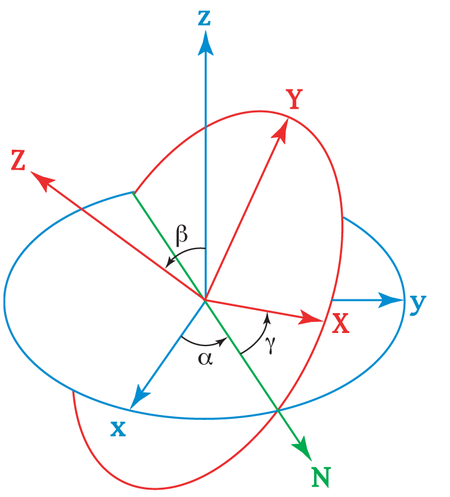
\includegraphics[width=0.9\linewidth]{img/eu_angles.png}
  \end{center}
    \caption{Углы Эйлера}
\end{wrapfigure}

Ортогональность матрицы $R$ даёт возможность описать её тремя независимыми параметрами. Один из вариантов сделать это -- углы Эйлера. 

Пусть начальная ПДСК $(x, y, z)$, а конечная -- $(X, Y, Z)$, при чём $xy \cap XY = ON$ -- линия узлов.
\begin{align*}
    1) \hspace{0.25cm}  \alpha &\colon Ox \to ON, &\text{ угол \textit{прецессии}}; \\
    2) \hspace{0.25cm}  \beta  &\colon Oz \to OZ, &\text{ угол \textit{нутации}}; \\
    3) \hspace{0.25cm}  \gamma &\colon OX \to ON, &\text{ угол \textit{собственного вращения}}.
\end{align*}
Повороты системы на эти углы называются прецессия, нутация и поворот на собственный угол (вращение). 

\phantom{42}

\noindent
Матричная запись углов Эйлера:
\begin{equation*}
    R_Z(\alpha) = \begin{pmatrix}
        \cos \alpha & - \sin \alpha & 0 \\
        \sin    a & \cos\alpha & 0 \\
        0 & 0 & 1\\
    \end{pmatrix},
\end{equation*}
\begin{equation*}
    R_X(\beta) = \begin{pmatrix}
        1 & 0 & 0 \\
        0 & \cos \beta & -\sin \beta \\
        0 & \sin \beta & \cos \beta \\
    \end{pmatrix},
    \hspace{1cm} 
    R_Z (\gamma) = \begin{pmatrix}
        \cos(\gamma) & - \sin \psi & 0 \\
        \sin \gamma & \cos \gamma & 0\\
        0 & 0 & 1
    \end{pmatrix}.
\end{equation*}

\begin{to_thr}[Теорема Эйлера]
     Произвольное перемещение твердого тела, имеющего неподвижную точку, можно осуществить посредством вращения вокруг некоторой оси, проходящей через эту точку. 
\end{to_thr}

\begin{to_thr}[Теорема Шаля]
     Самое общее перемещение твердого тела разлагается на поступательное перемещение, при котором произвольно выбранный полюс переходит из своего первоначального положения в конечное, и на вращение вокруг некоторой оси, проходящей через этот полюс. Это разложение можно совершить не единственным способом, выбирая за полюс различные точки тела; при этом направление и длина поступательного перемещения будут изменяться при выборе различных 
полюсов, а направление оси вращения и угол поворота вокруг нее не зависят от выбора полюса. 
\end{to_thr}

\begin{to_thr}[Теорема Моцци]
\label{thr_moz}
     Самое общее перемещение твердого тела является винтовым перемещением.
\end{to_thr}

\begin{to_con}[Теорема Бернулли-Шаля]
     Самое общее перемещение плоской фигуры в своей плоскости есть либо поступательное перемещение, либо вращение вокруг точки. Эта точка называется центром конечного вращения.
\end{to_con}